
\section{Introduction}
\label{sec.introduction}

This project is aiming to compare the accuracy of different approaches for
computing the principal square root of a Hermitian positive definite
matrix.
Throughout this work, we will always consider the principal square root.

\subsection{Outline}

We can compute the principal square root of any Hermitian
positive definite matrix via the following algorithm proposed by Higham
in~\ycite[2008, Alg.~6.21]{high08_fm}.
\begin{algorithm}[h]
\caption{Given a Hermitian positive definite matrix $A\in \C\nn$ this
  algorithm computes $H = A^{1/2}$.}
\label{alg:sqrt-higham}
\begin{algorithmic}[1]
\State{Compute the Cholesky factorization $A = R\tp R$.}
\State{Compute the Hermitian polar factor $H$ of $R$ by applying any method
  (exploiting the triangularity of $R$).} 
\end{algorithmic}
\end{algorithm}

Since we are focused on the Hermitian positive definite matrices, the Schur
decomposition of $A$ and its eigendecomposition coincide.
Therefore, we can simplify the Schur method, discussed in
Section~\ref{sec.schur-method}, and get 
\begin{algorithm}[h]
\caption{Given a Hermitian positive definite matrix $A\in \C\nn$ this
  algorithm computes $H = A^{1/2}$.} 
\label{alg:sqrt-eigdecomp}
\begin{algorithmic}[1]
\State{Compute the eigendecomposition $A = Q\varLambda Q\ctp$.}
\State{Compute the matrix square root $A^{1/2} = Q\varLambda^{1/2}Q\ctp$.}
\end{algorithmic}
\end{algorithm}

We would like to assess the accuracy of these two algorithms.
Suppose we are solving $H^{2} = A$, where $A,H\in\C\nn$, and are both
Hermitian positive definite. Let $\wh H_{1},\ \wh H_{2}$ be the computed
square root through Algorithm~\ref{alg:sqrt-higham}
and~\ref{alg:sqrt-eigdecomp}, respectively. We will compare the relative
forward and backward error defined by 
\begin{equation}\label{eq.fwd-bwd-errors}
  \text{forward error }\coloneqq \frac{\norm{H - \wh H_{i}}}{\norm{H}},
  \quad
  \text{backward error }\coloneqq \frac{\norm{A - \wh
  H_{i}^{2}}}{\norm{A}},
  \qquad
  i \in \{1,2\}.
\end{equation}
Clearly, the error depends on how we compute the Hermitian polar factor and
the eigendecomposition.
\begin{enumerate}
\item For Algorithm~\ref{alg:sqrt-higham}, we can compute the Hermitian
polar factor of $R$ using
\begin{enumerate}
\item Scaled Newton method \ycite[2008, Alg.~8.20]{high08_fm} or other
iterative approach. This can make use of the existing code by
Higham~\cite{high-mft}. 
\item The SVD approach. First compute the SVD $A = U\varSigma V\ctp$, and
then $H = V\varSigma V\ctp$.  
\end{enumerate}
\item For Algorithm~\ref{alg:sqrt-eigdecomp}, the eigendecomposition can be
computed by the MATLAB \inline{eig} command. More accurate method such
as the DV-SVD algorithm~\ycite[2008]{drve08i,drve08ii} will also be
consider but the numerical experiments will require Fortran.
\end{enumerate}

\subsection{Reproducible Research}
In this section, we will present our testing environment and system
specifications. All the experiments are conducted under the following
environment:
\begin{itemize}
\item MATLAB Version: 9.13.0.2126072 (R2022b) Update 3.
\item Device: Macbook Pro 13-inch, M1, 2020 Model, 16GB RAM, macOS Version
13.2.1.
\item The random number generator will be controlled by \inline{rng(1)}.
\end{itemize}

\subsection{Motivation}
The motivation of this work is based on the following experiment. We will
use the following functions,
\begin{itemize}
\item \inline{[U,H,k] = polar_newton(A)}: computes the polar decomposition
of $A$ by scaled Newton iteration~\cite{high-mft}.

\item \inline{[U,H] = polar_svd(A)}: computes the polar decomposition of
$A$ via singular value decomposition~\cite{high-mft}.

\item \inline{X = sqrtm(A)}: computes the principal square root of the
matrix $A$. This is a MATLAB built-in function\footnote{\inline{sqrtm}:
  \url{https://uk.mathworks.com/help/matlab/ref/sqrtm.html}}.


\item \inline{X = sqrt_chol_polar(A,method)}: computes the Hermitian
positive definite square root of a Hermitian positive definite matrix $A$
and with two options \inline{'newton'} and \inline{'svd'} to determine
using \inline{polar_newton} or \inline{polar_svd}.

\item \inline{A = gallery('randsvd',n,-kappa)}: generates a symmetric positive
definite matrix $A\in\R\nn$ with $\kappa_{2}(A) = \texttt{kappa}$.
\end{itemize}

The experiment will generate random Hermitian positive definite matrices
$X$ first, and computes $A = X^{2}$. Then, we apply both
Algorithm~\ref{alg:sqrt-higham} and \ref{alg:sqrt-eigdecomp} to $A$ and
obtain $\wh X_{1}$ and $\wh X_{2}$.
Finally, we compute the forward and backward error using
\eqref{eq.fwd-bwd-errors}. 

\begin{figure}[h]
\centering
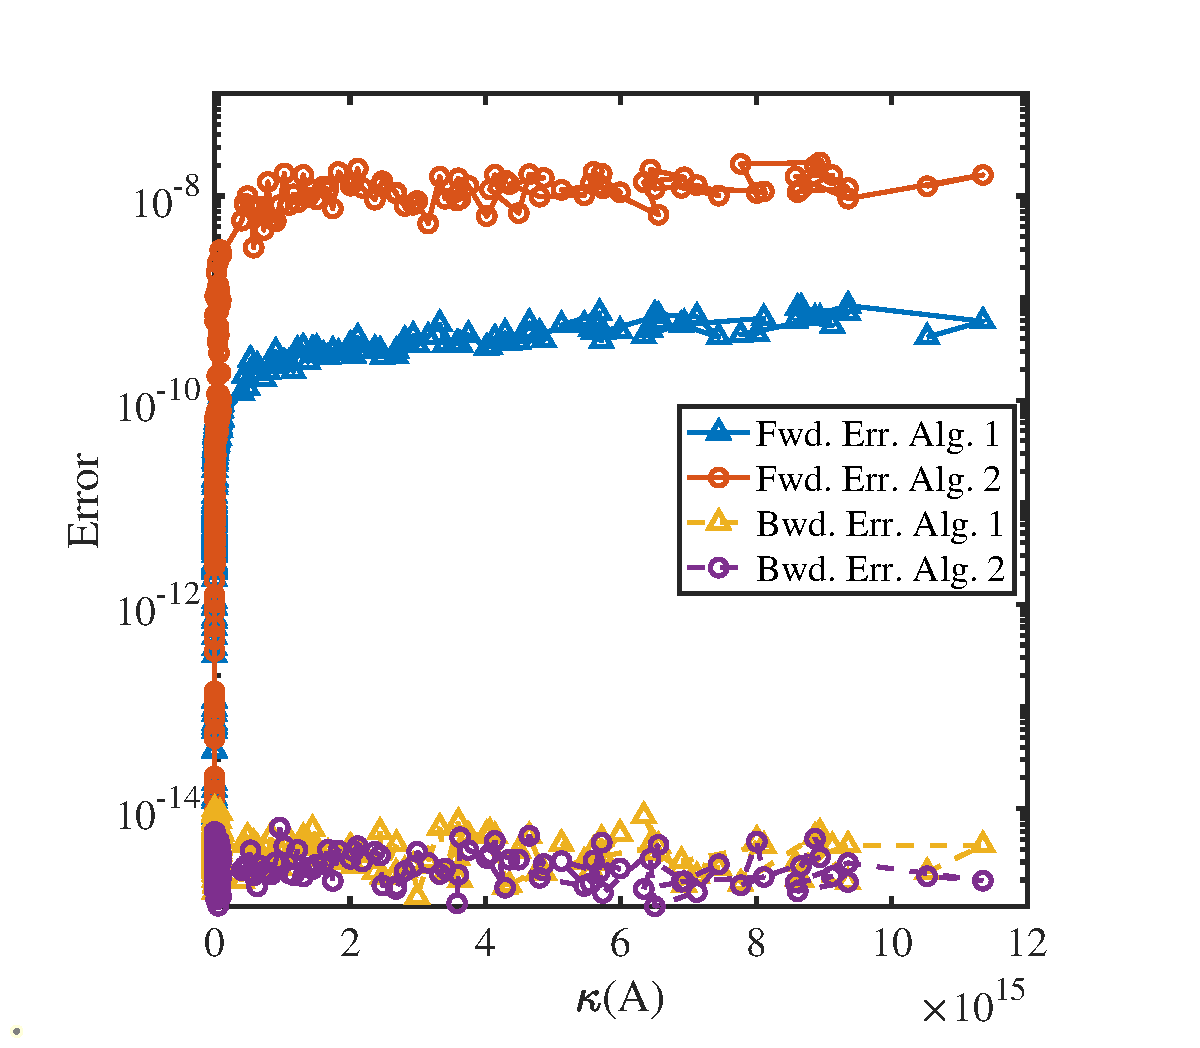
\includegraphics[width=0.6\textwidth]{figs/init_comp_svd_eig.eps}
\caption[Behavior of forward and backward errors of computed square
root.]{
  The forward errors and backward errors of
  Algorithm~\ref{alg:sqrt-higham} and \ref{alg:sqrt-eigdecomp} apply on a
  random Hermitian positive definite matrix $A\in\R^{100\times 100}$ with
  different condition numbers.
  The Hermitian polar factor is computed via SVD approach.
  For more detail, please refer to Appendix~\ref{app.init-compare}.}
\label{fig.init-compare-svd}
\end{figure}

\begin{figure}[h]
\centering
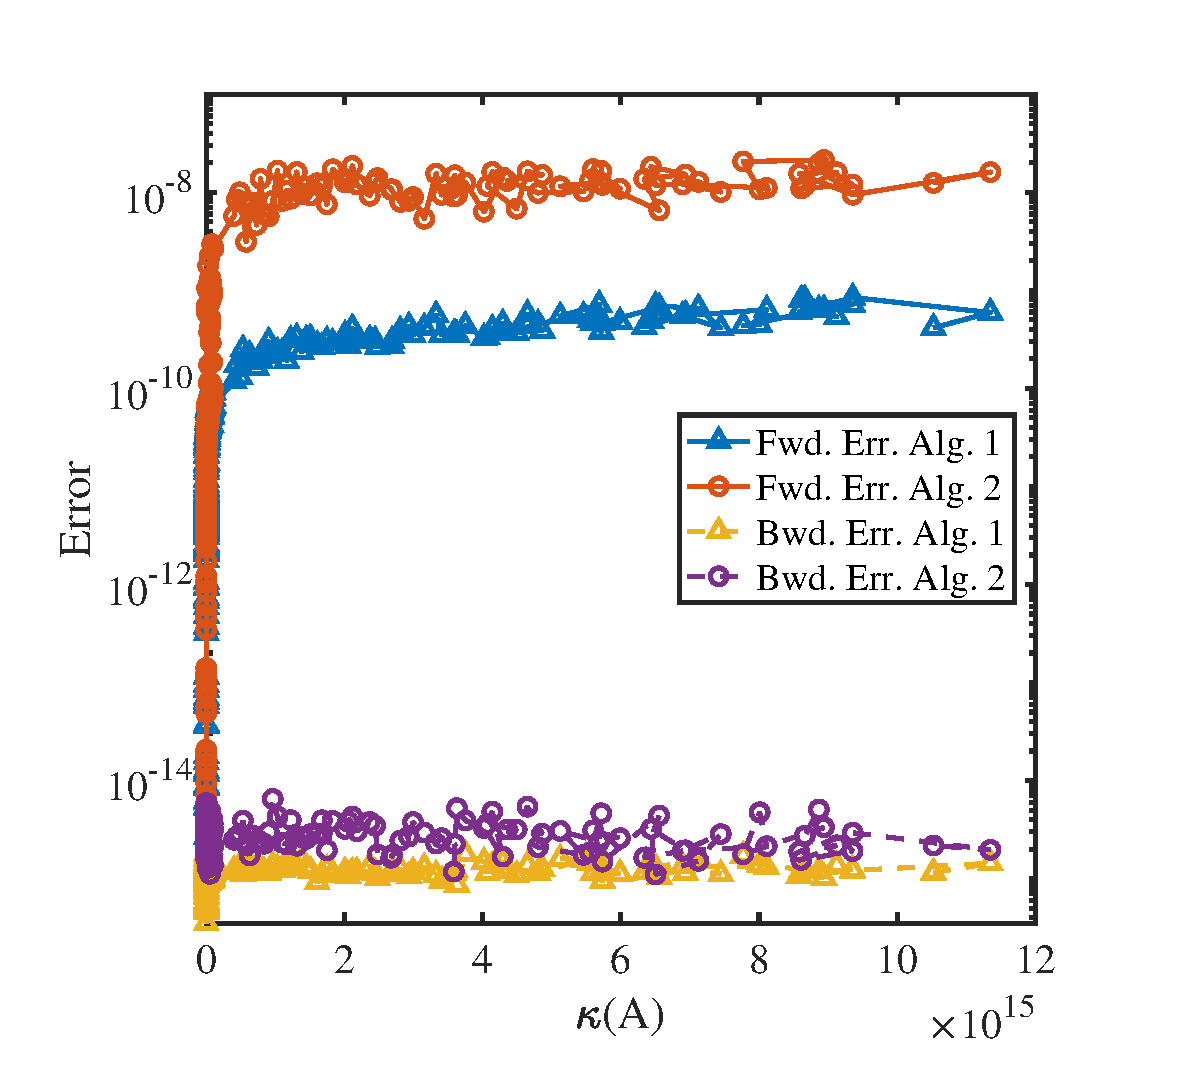
\includegraphics[width=0.6\textwidth]{figs/init_comp_newton_eig.eps}
\caption[Behavior of forward and backward errors of computed square
root.]{
  The forward errors and backward errors of
  Algorithm~\ref{alg:sqrt-higham} and \ref{alg:sqrt-eigdecomp} apply on a
  random Hermitian positive definite matrix $A\in\R^{100\times 100}$ with
  different condition numbers.
  The Hermitian polar factor is computed via iterative approach.
  For more detail, please refer to Appendix~\ref{app.init-compare}.}
\label{fig.init-compare-newton}
\end{figure}

Both Figure~\ref{fig.init-compare-svd} and \ref{fig.init-compare-newton}
show that the backward error is about the same regardless of the
conditioning of the problem. However, if we focus on the forward error,
$\norm{\wh X_{i} - X}/\norm{X}$, then for ill conditioned $A$, the
Algorithm~\ref{alg:sqrt-higham} will produce a square root that is 
significantly more accurate than the one computed by 
Algorithm~\ref{alg:sqrt-eigdecomp}. 



%%% Local Variables:
%%% mode: latex
%%% TeX-master: "do"
%%% End:
